%% 由 build/emit_tex.py 生成（生成物，勿手改）；定制请放 user_style.tex / user_meta.yaml
\chapter{第 4 章 ·
解析函数的级数表示法}\label{ux7b2c-4-ux7ae0-ux89e3ux6790ux51fdux6570ux7684ux7ea7ux6570ux8868ux793aux6cd5}

\section{4.1 复数项级数}\label{ux590dux6570ux9879ux7ea7ux6570}

\begin{quote}
本节目标：把实数项级数的极限、收敛、绝对收敛与条件收敛等概念平移到复数域，建立复数列极限与复级数收敛的判定方法。
重点：复数列极限与实、虚部分别收敛的等价关系；复级数收敛的充要条件与必要条件；绝对收敛与条件收敛。
难点：把复级数的收敛性归结为两个实级数；\(\sum a_n\) 收敛与
\(\sum |a_n|\) 收敛的区分。
\end{quote}

对应幻灯片：第 2--10 页。

\subsection{4.1.1
复数列和复数列的极限}\label{ux590dux6570ux5217ux548cux590dux6570ux5217ux7684ux6781ux9650}

\textbf{定义 4.1} 设 \(\{a_n\}(n=1,2,\cdots)\) 为一复数列，其中

\[
a_n=\alpha_n+\mathrm{i}\beta_n,
\]

\(a=\alpha+\mathrm{i}\beta\) 为一确定的复数。如果对任意的正数
\(\varepsilon\)，存在正整数 \(N\)，使得当 \(n>N\) 时，有

\[
|a_n-a|<\varepsilon
\]

成立，则称 \(a\) 为复数列 \(\{a_n\}\) 当 \(n\to\infty\) 时的极限，记作

\[
\lim_{n\to\infty} a_n=a,
\]

并称复数列 \(\{a_n\}\) 收敛于 \(a\)。

\textbf{定理 4.1} 复数列 \(\{a_n\}\) 收敛于 \(a\) 的充分必要条件是

\[
\lim_{n\to\infty}\alpha_n=\alpha,\qquad \lim_{n\to\infty}\beta_n=\beta .
\]

\textbf{证明要点}

\begin{itemize}
\tightlist
\item
  必要性：若 \(\lim a_n=a\)，则对 \(\varepsilon>0\)，存在正整数
  \(N\)，使当 \(n>N\) 时 \(|a_n-a|<\varepsilon\)。从而
\end{itemize}

\[
|\alpha_n-\alpha|\le|a_n-a|<\varepsilon,
\]

故 \(\lim\alpha_n=\alpha\)；同理有 \(\lim\beta_n=\beta\)。

\begin{itemize}
\tightlist
\item
  充分性：若 \(\lim\alpha_n=\alpha\)，\(\lim\beta_n=\beta\)，对
  \(\varepsilon>0\)，存在正整数 \(N\)，使当 \(n>N\) 时
\end{itemize}

\[
|\alpha_n-\alpha|<\frac{\varepsilon}{2},\qquad |\beta_n-\beta|<\frac{\varepsilon}{2},
\]

于是

\[
|a_n-a|\le|\alpha_n-\alpha|+|\beta_n-\beta|<\varepsilon,
\]

故 \(\lim a_n=a\)。

\(\square\)

\subsection{4.1.2 复级数}\label{ux590dux7ea7ux6570}

设 \(\{a_n\}\) 为一复数列，表达式

\[
\sum_{n=1}^{\infty}a_n=a_1+a_2+\cdots+a_n+\cdots
\]

称为复数域上的无穷级数，简称复级数或级数。记该级数的前 \(n\) 项部分和为

\[
s_n=a_1+a_2+\cdots+a_n=\sum_{i=1}^{n}a_i,\qquad (n=1,2,\cdots),
\]

\(\{s_n\}\) 称为该级数的部分和数列。

\textbf{定义 4.2} 若级数 \(\displaystyle\sum_{n=1}^{\infty}a_n\)
对应的部分和数列 \(\{s_n\}\) 收敛于常数 \(s\)，即

\[
\lim_{n\to\infty}s_n=s,
\]

那么 \(\displaystyle\sum_{n=1}^{\infty}a_n\) 称为收敛的级数，数 \(s\)
叫做该级数的和，记为

\[
\sum_{n=1}^{\infty}a_n=s.
\]

若 \(\lim s_n\) 不存在，则称该级数为发散的级数。

\textbf{定理 4.2} 复级数 \(\displaystyle\sum_{n=1}^{\infty}a_n\) 收敛于
\(s\) 的充要条件是实级数 \(\displaystyle\sum_{n=1}^{\infty}\alpha_n\) 和
\(\displaystyle\sum_{n=1}^{\infty}\beta_n\) 分别收敛于 \(\delta\) 和
\(\tau\)，其中

\[
s=\delta+\mathrm{i}\tau,\qquad a_n=\alpha_n+\mathrm{i}\beta_n\ (n=1,2,\cdots).
\]

\textbf{证明要点}

\[
s_n=a_1+a_2+\cdots+a_n=(\alpha_1+\alpha_2+\cdots+\alpha_n)+\mathrm{i}(\beta_1+\beta_2+\cdots+\beta_n)=\delta_n+\mathrm{i}\tau_n,
\]

其中

\[
\delta_n=\sum_{i=1}^{n}\alpha_i,\qquad \tau_n=\sum_{i=1}^{n}\beta_i ,
\]

它们分别为实级数 \(\sum\alpha_i\) 和 \(\sum\beta_i\)（即
\(\sum\alpha_n\)、\(\sum\beta_n\)）的部分和。

由定义 4.2 及定理 4.1 知，\(s_n\) 收敛于 \(s\) 的充要条件是
\(\{\delta_n\}\) 和 \(\{\tau_n\}\) 分别收敛于 \(\delta\) 和
\(\tau\)，从而定理得证。\(\square\)

\textbf{定理 4.3} 复级数 \(\displaystyle\sum_{n=1}^{\infty}a_n\)
收敛的必要条件是

\[
\lim_{n\to\infty}a_n=0 .
\]

\textbf{证明要点} 级数 \(\sum a_n\) 收敛的充要条件是实级数
\(\sum\alpha_n\) 和 \(\sum\beta_n\)
均收敛。实级数收敛的必要条件是其通项的极限为零，即

\[
\lim_{n\to\infty}\alpha_n=0,\qquad \lim_{n\to\infty}\beta_n=0,
\]

从而得到

\[
\lim_{n\to\infty}a_n=0 .
\]

\(\square\)

\textbf{定义 4.3} 对于复级数 \(\displaystyle\sum_{n=1}^{\infty}a_n\)：

\begin{itemize}
\tightlist
\item
  若 \(\displaystyle\sum_{n=1}^{\infty}|a_n|\)
  收敛，则称级数\textbf{绝对收敛}；
\item
  若 \(\displaystyle\sum_{n=1}^{\infty}|a_n|\) 发散，而
  \(\displaystyle\sum_{n=1}^{\infty}a_n\)
  收敛，则称级数\textbf{条件收敛}。
\end{itemize}

\textbf{定理 4.4} 如果级数 \(\displaystyle\sum_{n=1}^{\infty}a_n\)
绝对收敛，则 \(\displaystyle\sum_{n=1}^{\infty}a_n\) 也收敛，且不等式

\[
\left|\sum_{n=1}^{\infty}a_n\right|\le\sum_{n=1}^{\infty}|a_n|
\]

成立。

\textbf{证明要点} 记 \(a_n=\alpha_n+\mathrm{i}\beta_n\)，则

\[
\sum_{n=1}^{\infty}|a_n|=\sum_{n=1}^{\infty}\sqrt{\alpha_n^2+\beta_n^2}.
\]

由于

\[
|\alpha_n|\le\sqrt{\alpha_n^2+\beta_n^2},\qquad |\beta_n|\le\sqrt{\alpha_n^2+\beta_n^2},
\]

所以实级数 \(\sum\alpha_n\) 和 \(\sum\beta_n\) 均收敛，于是 \(\sum a_n\)
收敛。再由部分和取极限并结合三角不等式即得上述不等式。\(\square\)

\textbf{推论 4.1} 设
\(a_n=\alpha_n+\mathrm{i}\beta_n\ (n=1,2,\cdots)\)。则级数
\(\displaystyle\sum_{n=1}^{\infty}a_n\) 绝对收敛的充要条件是级数
\(\displaystyle\sum_{n=1}^{\infty}\alpha_n\) 和
\(\displaystyle\sum_{n=1}^{\infty}\beta_n\) 都绝对收敛。

\subsection{4.1.3 例题}\label{ux4f8bux9898-1}

\textbf{例 4.1} 下列级数是否收敛？是否绝对收敛？

\[
(1)\ \sum_{n=1}^{\infty}\frac{(3\mathrm{i})^n}{n!};\qquad
(2)\ \sum_{n=1}^{\infty}\left(1+\frac{1}{n}\right)\mathrm{e}^{\mathrm{i}\pi/n};\qquad
(3)\ \sum_{n=1}^{\infty}\left[\frac{(-1)^n}{n}+\frac{1}{3^n}\mathrm{i}\right].
\]

\textbf{解}

\textbf{(1)}
\(\left|\dfrac{(3\mathrm{i})^n}{n!}\right|=\dfrac{3^n}{n!}\)。由正项级数的比值判别法知
\(\displaystyle\sum_{n=1}^{\infty}\frac{3^n}{n!}\)
收敛，故原级数为绝对收敛。

\textbf{(2)} 由欧拉公式，

\[
\left(1+\frac{1}{n}\right)\mathrm{e}^{\mathrm{i}\pi/n}=\left(1+\frac{1}{n}\right)\cos\frac{\pi}{n}+\mathrm{i}\left(1+\frac{1}{n}\right)\sin\frac{\pi}{n}.
\]

而

\[
\lim_{n\to\infty}\left(1+\frac{1}{n}\right)\cos\frac{\pi}{n}=1,\qquad
\lim_{n\to\infty}\left(1+\frac{1}{n}\right)\sin\frac{\pi}{n}=0,
\]

所以

\[
\lim_{n\to\infty}\left(1+\frac{1}{n}\right)\mathrm{e}^{\mathrm{i}\pi/n}=1\neq 0 .
\]

故级数
\(\displaystyle\sum_{n=1}^{\infty}\left(1+\frac{1}{n}\right)\mathrm{e}^{\mathrm{i}\pi/n}\)
发散。

\textbf{(3)} 因为 \(\displaystyle\sum_{n=1}^{\infty}\frac{(-1)^n}{n}\)
收敛（且为条件收敛），\(\displaystyle\sum_{n=1}^{\infty}\frac{1}{3^n}\)
也收敛，故原级数收敛。但
\(\displaystyle\sum_{n=1}^{\infty}\left|\frac{(-1)^n}{n}\right|=\sum_{n=1}^{\infty}\frac{1}{n}\)
发散，故原级数为条件收敛。

\subsection{常见错误与注意点}\label{ux5e38ux89c1ux9519ux8befux4e0eux6ce8ux610fux70b9-11}

\begin{itemize}
\tightlist
\item
  不要把``\(\sum a_n\) 收敛''与``\(\sum|a_n|\)
  收敛''混为一谈：前者收敛只能说明通项趋于零，不能保证绝对收敛；\(\sum|a_n|\)
  收敛才保证 \(\sum a_n\) 收敛。
\item
  定理 4.3 只是必要条件：\(\lim a_n=0\) 不能推出 \(\sum a_n\) 收敛。
\item
  判断复级数敛散时，优先把 \(a_n\) 拆成实部 \(\alpha_n\) 与虚部
  \(\beta_n\)，转化为两个实级数来处理。
\item
  例 4.1(2) 属于``通项不趋于零''的情形，是最常用的发散判定。
\end{itemize}

\subsection{本节小结}\label{ux672cux8282ux5c0fux7ed3-11}

\begin{itemize}
\tightlist
\item
  复数列收敛 \(\iff\) 实部、虚部分别收敛（定理
  4.1），从而可用实数极限理论处理复数列。
\item
  复级数由部分和数列 \(\{s_n\}\) 的敛散定义（定义 4.2）；其收敛 \(\iff\)
  实、虚部两个实级数分别收敛（定理 4.2）。
\item
  通项趋于零是复级数收敛的必要条件（定理 4.3）。
\item
  绝对收敛 \(\Rightarrow\) 收敛，且 \(|\sum a_n|\le\sum|a_n|\)（定理
  4.4）；\(\sum a_n\) 绝对收敛 \(\iff\) \(\sum\alpha_n\) 与
  \(\sum\beta_n\) 都绝对收敛（推论 4.1）。
\end{itemize}

\section{4.2 幂级数}\label{ux5e42ux7ea7ux6570}

\begin{quote}
本节目标：掌握幂级数的概念、收敛域（收敛半径、收敛圆）、收敛半径的比值法与根值法，以及幂级数在收敛圆内的解析性（逐项求导、逐项积分）。
重点：收敛半径的两种求法（定理
4.6、4.7）；幂级数在收敛圆内解析、可逐项求导与逐项积分的性质。
难点：收敛半径的意义、\(|z|=R\)
边界上的敛散性、两个幂级数``运算后半径不小于
\(\min\{R_1,R_2\}\)''的理解；幂级数乘法（Cauchy 乘积）的收敛范围。
\end{quote}

对应幻灯片：第 11--24 页。

\subsection{4.2.1
幂级数的概念}\label{ux5e42ux7ea7ux6570ux7684ux6982ux5ff5}

\textbf{幂级数}是指形如

\[
\sum_{n=0}^{\infty} a_n(z-z_0)^n=a_0+a_1(z-z_0)+a_2(z-z_0)^2+\cdots+a_n(z-z_0)^n+\cdots
\]

的表达式，它的一般项是幂函数 \(a_n(z-z_0)^n\)，这里
\(a_n\ (n=0,1,\cdots)\) 和 \(z_0\) 是复常数，而 \(z\) 为复变数。

给定 \(z\) 的一个确定值 \(z_1\)，则

\[
\sum_{n=0}^{\infty}a_n(z_1-z_0)^n=a_0+a_1(z_1-z_0)+a_2(z_1-z_0)^2+\cdots
\]

为复数项级数。若该复数项级数收敛，则称幂级数在 \(z_1\) 处收敛，\(z_1\)
称为幂级数的一个收敛点；否则称为发散点。

若 \(D\) 为幂级数所有收敛点的集合，则级数在 \(D\) 上的和确定一个函数
\(s(z)\)：

\[
s(z)=\sum_{n=0}^{\infty}a_n z^n=a_0+a_1 z+a_2 z^2+\cdots+a_n z^n+\cdots,
\]

称 \(s(z)\) 为幂级数的\textbf{和函数}。特别地，假定
\(z_0=0\)，幂级数成为

\[
\sum_{n=0}^{\infty}a_n z^n=a_0+a_1 z+a_2 z^2+\cdots+a_n z^n+\cdots .
\]

\subsection{4.2.2
收敛半径和收敛圆}\label{ux6536ux655bux534aux5f84ux548cux6536ux655bux5706}

\textbf{定理 4.5} 如果幂级数 \(\displaystyle\sum_{n=0}^{\infty}a_n z^n\)
在 \(z=z_1(\neq 0)\) 处收敛，则对于满足 \(|z|<|z_1|\) 的
\(z\)，级数必绝对收敛；如果在 \(z=z_2\) 处级数发散，则对于 \(|z|>|z_2|\)
的 \(z\)，级数必发散。

\textbf{证明要点} 由于 \(\sum a_n z_1^n\) 级数收敛，有
\(\lim_{n\to\infty}a_n z_1^n=0\)，因而存在正数 \(M\)，使对所有的 \(n\)
成立 \(|a_n z_1^n|<M\)。

如果 \(|z|<|z_1|\)，那么 \(\left|\dfrac{z}{z_1}\right|=q<1\)，而

\[
|a_n z^n|=|a_n z_1^n|\cdot\left|\frac{z}{z_1}\right|^n<Mq^n .
\]

由于 \(\sum Mq^n\) 是公比小于 \(1\) 的等比数列，故收敛，于是
\(\sum|a_n z^n|\) 收敛，从而级数 \(\sum a_n z^n\) 绝对收敛。

对``在 \(z_2\) 发散''的情形，用反证法：若存在 \(|z|>|z_2|\)
使级数收敛，则由已证部分会推出在 \(z_2\) 处也收敛，矛盾。\(\square\)

幂级数 \(\displaystyle\sum_{n=0}^{\infty}a_n z^n\) 的收敛情况只有三种：

\begin{enumerate}
\def\labelenumi{\arabic{enumi}.}
\tightlist
\item
  除 \(z=0\) 外，级数处处发散；
\item
  对于所有 \(z\) 级数都收敛，级数在复平面内处处绝对收敛；
\item
  存在一个正实数 \(R\)，使级数在 \(|z|<R\) 中收敛，在 \(|z|>R\) 中发散。
\end{enumerate}

该正实数 \(R\) 称为级数的\textbf{收敛半径}，以原点为中心、半径为 \(R\)
的圆盘称为级数的\textbf{收敛圆}。对幂级数
\(\displaystyle\sum_{n=0}^{\infty}a_n(z-z_0)^n\) 来说，它的收敛圆是以
\(z_0\) 为中心的圆盘 \(|z-z_0|<R\)。

\begin{figure}
\centering
\pandocbounded{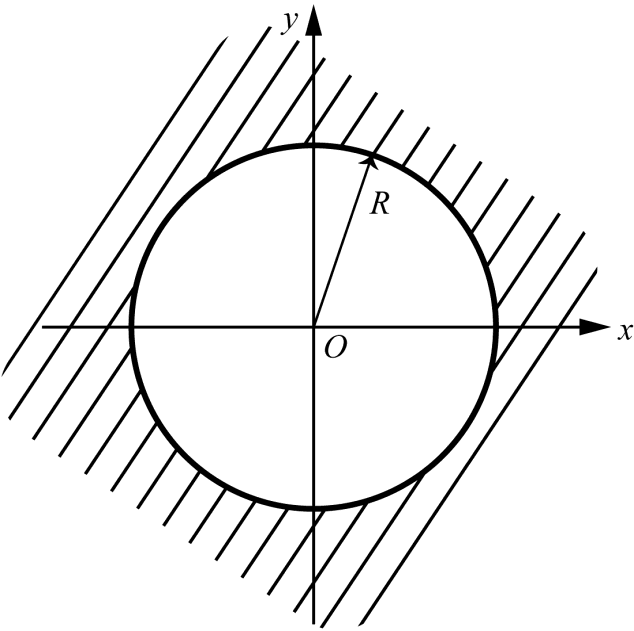
\includegraphics[keepaspectratio,alt={图4.1 幂级数的收敛圆}]{figures/04-解析函数的级数表示法/fig-p14-02b5ec75.png}}
\caption{图4.1 幂级数的收敛圆}
\end{figure}

\textbf{例 4.2} 讨论幂级数

\[
\sum_{n=0}^{\infty}z^n=1+z+z^2+\cdots+z^n+\cdots
\]

的收敛范围与和函数。

\textbf{解} 级数的部分和为

\[
s_n(z)=
\begin{cases}
\dfrac{1-z^n}{1-z}, & z\neq 1,\\[4pt]
n, & z=1.
\end{cases}
\]

该级数的收敛半径为 \(1\)，收敛圆为 \(|z|<1\)，且级数在圆周 \(|z|=1\)
上处处发散。于是

\[
\lim_{n\to\infty}s_n(z)=
\begin{cases}
\dfrac{1}{1-z}, & |z|<1,\\[4pt]
\text{发散}, & |z|\ge 1.
\end{cases}
\]

即和函数 \(s(z)=\dfrac{1}{1-z}\ (|z|<1)\)。

\subsection{4.2.3
收敛半径的求法}\label{ux6536ux655bux534aux5f84ux7684ux6c42ux6cd5}

\textbf{定理 4.6} 若 \(\displaystyle\sum_{n=0}^{\infty}a_n z^n\)
的系数满足

\[
\lim_{n\to\infty}\left|\frac{a_{n+1}}{a_n}\right|=\rho ,
\]

则

\begin{enumerate}
\def\labelenumi{\arabic{enumi}.}
\tightlist
\item
  当 \(0<\rho<+\infty\) 时，\(R=\dfrac{1}{\rho}\)；
\item
  当 \(\rho=0\) 时，\(R=+\infty\)（处处收敛）；
\item
  当 \(\rho=+\infty\) 时，\(R=0\)（仅有一个收敛点 \(z=0\)）。
\end{enumerate}

\textbf{证明要点} 考虑正项级数

\[
\sum_{n=0}^{\infty}|a_n z^n|=|a_0|+|a_1 z|+\cdots+|a_n z^n|+\cdots,
\]

其相邻项之比

\[
\lim_{n\to\infty}\left|\frac{a_{n+1}z^{n+1}}{a_n z^n}\right|=\rho|z| .
\]

\begin{itemize}
\tightlist
\item
  若 \(0<\rho<+\infty\)，由正项级数的比值判别法知，当 \(\rho|z|<1\)（即
  \(|z|<\frac{1}{\rho}\)）时 \(\sum|a_n z^n|\) 收敛，从而
  \(\sum a_n z^n\) 收敛；当 \(\rho|z|>1\)（即 \(|z|>\frac{1}{\rho}\)）时
  \(\lim\left|\frac{a_{n+1}z^{n+1}}{a_n z^n}\right|>1\)，故当 \(n\)
  充分大时 \(|a_{n+1}z^{n+1}|\ge|a_n z^n|\)，所以当 \(n\to\infty\)
  时一般项 \(a_n z^n\) 不能趋于零，级数发散。故收敛半径
  \(R=\frac{1}{\rho}\)。
\item
  若 \(\rho=0\)，则 \(\rho|z|<1\) 对任何 \(z\) 成立，故对任何 \(z\) 级数
  \(\sum|a_n z^n|\) 收敛（即处处绝对收敛），收敛半径 \(R=+\infty\)。
\item
  若 \(\rho=+\infty\)，对任意 \(z\neq 0\)，当 \(n\) 充分大时必有
  \(|a_{n+1}z^{n+1}|\ge|a_n z^n|\)，由此得 \(\sum a_n z^n\)
  发散，故收敛半径 \(R=0\)。\(\square\)
\end{itemize}

\textbf{定理 4.7} 若幂级数 \(\displaystyle\sum_{n=0}^{\infty}a_n z^n\)
的系数满足

\[
\lim_{n\to\infty}\sqrt[n]{|a_n|}=\rho ,
\]

则

\begin{enumerate}
\def\labelenumi{\arabic{enumi}.}
\tightlist
\item
  当 \(0<\rho<+\infty\) 时，\(R=\dfrac{1}{\rho}\)；
\item
  当 \(\rho=0\) 时，\(R=+\infty\)；
\item
  当 \(\rho=+\infty\) 时，\(R=0\)。
\end{enumerate}

\subsection{4.2.4
幂级数的运算及性质}\label{ux5e42ux7ea7ux6570ux7684ux8fd0ux7b97ux53caux6027ux8d28}

\textbf{性质 4.1} 若幂级数 \(\displaystyle\sum_{n=0}^{\infty}a_n z^n\)
和 \(\displaystyle\sum_{n=0}^{\infty}b_n z^n\) 的收敛半径分别为 \(R_1\)
和 \(R_2\)，则幂级数 \(\displaystyle\sum_{n=0}^{\infty}(a_n\pm b_n)z^n\)
的收敛半径不小于

\[
R=\min\{R_1,R_2\},
\]

且在 \(|z|<R\) 内有

\[
\sum_{n=0}^{\infty}a_n z^n\pm\sum_{n=0}^{\infty}b_n z^n=\sum_{n=0}^{\infty}(a_n\pm b_n)z^n .
\]

\textbf{性质 4.2} 若幂级数 \(\displaystyle\sum_{n=0}^{\infty}a_n z^n\)
和 \(\displaystyle\sum_{n=0}^{\infty}b_n z^n\) 的收敛半径分别为 \(R_1\)
和 \(R_2\)，则幂级数（Cauchy 乘积）

\[
a_0b_0+(a_0b_1+a_1b_0)z+(a_0b_2+a_1b_1+a_2b_0)z^2+\cdots+\left(\sum_{i=0}^{n}a_i b_{n-i}\right)z^n+\cdots
\]

的收敛半径不小于 \(R=\min\{R_1,R_2\}\)，且在 \(|z|<R\) 内有

\[
\left(\sum_{n=0}^{\infty}a_n z^n\right)\cdot\left(\sum_{n=0}^{\infty}b_n z^n\right)=\sum_{n=0}^{\infty}\left(\sum_{i=0}^{n}a_i b_{n-i}\right)z^n .
\]

\textbf{例 4.3} 设有幂级数 \(\displaystyle\sum_{n=0}^{\infty}z^n\) 与
\(\displaystyle\sum_{n=0}^{\infty}\frac{1}{1+a^n}z^n\)（\(0<a<1\)），求

\[
\sum_{n=0}^{\infty}\left(1-\frac{1}{1+a^n}\right)z^n=\sum_{n=0}^{\infty}\frac{a^n}{1+a^n}z^n
\]

的收敛半径。

\textbf{解} \(\displaystyle\sum_{n=0}^{\infty}z^n\) 和
\(\displaystyle\sum_{n=0}^{\infty}\frac{1}{1+a^n}z^n\) 的收敛半径都为
\(1\)，而

\[
\sum_{n=0}^{\infty}\frac{a^n}{1+a^n}z^n
\]

的收敛半径为 \(\dfrac{1}{a}\ (>1)\)。但等式

\[
\sum_{n=0}^{\infty}z^n-\sum_{n=0}^{\infty}\frac{1}{1+a^n}z^n=\sum_{n=0}^{\infty}\left(1-\frac{1}{1+a^n}\right)z^n
\]

成立的范围仍为 \(|z|<1\)。当 \(1\le|z|<\frac{1}{a}\)
时，等式左边的两个级数都不收敛，所以等式没有意义。

\subsection{4.2.5
幂级数的解析性（逐项求导与逐项积分）}\label{ux5e42ux7ea7ux6570ux7684ux89e3ux6790ux6027ux9010ux9879ux6c42ux5bfcux4e0eux9010ux9879ux79efux5206}

\textbf{定理 4.8} 设幂级数
\(\displaystyle\sum_{n=0}^{\infty}a_n(z-z_0)^n\) 的收敛半径为
\(R\)，那么

\begin{enumerate}
\def\labelenumi{\arabic{enumi}.}
\tightlist
\item
  它的和函数 \(\displaystyle f(z)=\sum_{n=0}^{\infty}a_n(z-z_0)^n\)
  在收敛圆 \(|z-z_0|<R\) 内是解析函数；
\item
  \(f(z)\) 的导数可通过对其幂级数逐项求导得到，即
\end{enumerate}

\[
f'(z)=\sum_{n=0}^{\infty}n a_n(z-z_0)^{n-1}\qquad (|z-z_0|<R);
\]

\begin{enumerate}
\def\labelenumi{\arabic{enumi}.}
\setcounter{enumi}{2}
\tightlist
\item
  \(f(z)\) 在 \(|z-z_0|<R\) 内可以逐项积分，即
\end{enumerate}

\[
\int_C f(z)\,\mathrm{d}z=\sum_{n=0}^{\infty}a_n\int_C(z-z_0)^n\,\mathrm{d}z,
\]

其中 \(C\) 为 \(|z-z_0|<R\) 内的曲线。

\textbf{例 4.4} 求出下列幂级数的和函数。

\[
(1)\ \sum_{n=1}^{\infty}(2^n-1)z^{n-1};\qquad
(2)\ \sum_{n=0}^{\infty}(n+1)z^n .
\]

\textbf{解}

\textbf{(1)}
\(\displaystyle\lim_{n\to\infty}\left|\frac{a_{n+1}}{a_n}\right|=\lim_{n\to\infty}\frac{|2^{n+1}-1|}{|2^n-1|}=2\)，故收敛半径为
\(R=\dfrac{1}{2}\)。同样 \(\sum_{n=1}^{\infty}2^n z^{n-1}\) 和
\(\sum_{n=1}^{\infty}z^{n-1}\) 的收敛半径分别为 \(R_1=\dfrac{1}{2}\) 和
\(R_2=1\)。

当 \(|z|<\dfrac{1}{2}\) 时，

\[
\sum_{n=1}^{\infty}(2^n-1)z^{n-1}=\sum_{n=1}^{\infty}2^n z^{n-1}-\sum_{n=1}^{\infty}z^{n-1}
=2\sum_{n=1}^{\infty}(2z)^{n-1}-\sum_{n=1}^{\infty}z^{n-1}
\]

\[
=2\cdot\frac{1}{1-2z}-\frac{1}{1-z}=\frac{1}{(1-2z)(1-z)} .
\]

\textbf{(2)}
\(\displaystyle\lim_{n\to\infty}\left|\frac{a_{n+1}}{a_n}\right|=\lim_{n\to\infty}\frac{n+2}{n+1}=1\)，故收敛半径为
\(R=1\)。

在 \(|z|<1\) 内取一条连接 \(0\) 和 \(z\) 的简单曲线
\(C\)，由逐项积分性质，得

\[
\int_0^z\sum_{n=0}^{\infty}(n+1)w^n\,\mathrm{d}w=\sum_{n=0}^{\infty}\int_0^z(n+1)w^n\,\mathrm{d}w=\sum_{n=0}^{\infty}z^{n+1}=\frac{z}{1-z},\qquad |z|<1 .
\]

再对两边求导，得

\[
\sum_{n=0}^{\infty}(n+1)z^n=\left(\frac{z}{1-z}\right)'=\frac{1}{(1-z)^2},\qquad |z|<1 .
\]

\subsection{常见错误与注意点}\label{ux5e38ux89c1ux9519ux8befux4e0eux6ce8ux610fux70b9-12}

\begin{itemize}
\tightlist
\item
  收敛半径只保证 \(|z|<R\) 内收敛；边界 \(|z|=R\)
  上的点可能收敛、也可能发散，必须另行判断。
\item
  定理 4.6、4.7 中 \(\rho\) 是\textbf{非负实数}，不要漏掉
  \(\rho=0\)、\(\rho=+\infty\) 两种极限情形。
\item
  幂级数做加减、乘法后，收敛半径只保证``不小于
  \(\min\{R_1,R_2\}\)''，实际半径可能更大（见例
  4.3），但在两个原级数都不收敛的区域内，用``和/差''表示的等式不成立。
\item
  逐项求导、逐项积分都在收敛圆内（开圆盘）进行，不能越过收敛圆周。
\end{itemize}

\subsection{本节小结}\label{ux672cux8282ux5c0fux7ed3-12}

\begin{itemize}
\tightlist
\item
  幂级数 \(\sum a_n(z-z_0)^n\) 的收敛域是以 \(z_0\)
  为中心的圆盘（或全平面、仅一点），边界敛散不定（§4.2.2）。
\item
  收敛半径可由比值法 \(\rho=\lim|a_{n+1}/a_n|\) 或根值法
  \(\rho=\lim\sqrt[n]{|a_n|}\) 求得，\(R=1/\rho\)（定理 4.6、4.7）。
\item
  两幂级数之和、积在 \(|z|<\min\{R_1,R_2\}\)
  上成立，且和/积级数的半径不小于该值（性质 4.1、4.2）。
\item
  收敛圆内和函数解析，可逐项求导、逐项积分（定理
  4.8），这是求幂级数和函数及泰勒展开的基础。
\end{itemize}

\section{4.3
解析函数的泰勒展开}\label{ux89e3ux6790ux51fdux6570ux7684ux6cf0ux52d2ux5c55ux5f00}

\begin{quote}
本节目标：理解解析函数在圆盘内可展开成幂级数（泰勒级数）这一基本定理，掌握展开式的唯一性、解析与有泰勒展式的等价关系、零点及其阶数判定，并牢记常用初等函数的泰勒展开式。
重点：泰勒定理（定理 4.9）及其思想；展开式唯一性；零点的阶数（\(m\)
阶零点）；\(\mathrm{e}^z\)、\(\cos z\)、\(\sin z\) 的展开。
难点：泰勒定理证明中柯西积分公式与几何级数展开、余项估计的思想；零点阶数与导数条件（性质
4.4）。
\end{quote}

对应幻灯片：第 25--32 页。

\subsection{4.3.1 泰勒定理}\label{ux6cf0ux52d2ux5b9aux7406}

\textbf{定理 4.9} 设 \(K\) 表示以 \(z_0\) 为中心、半径为 \(r\)
的一个圆，\(f(z)\) 在 \(K\) 内解析，则 \(f(z)\) 可以在 \(K\)
内展开成幂级数，即

\[
f(z)=\sum_{n=0}^{\infty}\frac{f^{(n)}(z_0)}{n!}(z-z_0)^n,\qquad z\in K .
\]

并称它为 \(f(z)\) 在 \(z_0\) 的泰勒（Taylor）展开式，上式右端的级数称为
\(f(z)\) 的泰勒级数。

\begin{figure}
\centering
\pandocbounded{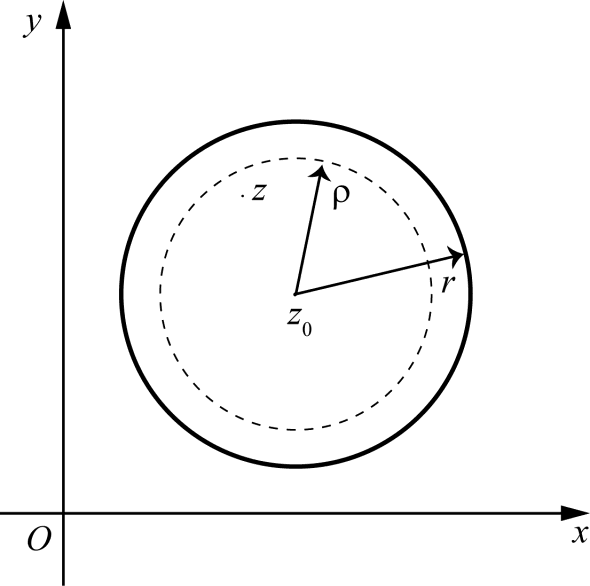
\includegraphics[keepaspectratio,alt={图4.2 泰勒展开的证明示意}]{figures/04-解析函数的级数表示法/fig-p25-54aa3acd.png}}
\caption{图4.2 泰勒展开的证明示意}
\end{figure}

\textbf{证明要点}

\begin{enumerate}
\def\labelenumi{\arabic{enumi}.}
\tightlist
\item
  任意取定 \(z\in K\)，再取正数 \(\rho\)，使 \(\rho<r\)，且
  \(|z-z_0|<\rho\)，即圆 \(|\zeta-z_0|=\rho\) 在 \(K\)
  内。根据柯西积分公式，得
\end{enumerate}

\[
f(z)=\frac{1}{2\pi\mathrm{i}}\oint_{|\zeta-z_0|=\rho}\frac{f(\zeta)}{\zeta-z}\,\mathrm{d}\zeta .
\]

\begin{enumerate}
\def\labelenumi{\arabic{enumi}.}
\setcounter{enumi}{1}
\tightlist
\item
  把 \(\dfrac{1}{\zeta-z}\) 按 \(|z-z_0|<|\zeta-z_0|\) 展开成几何级数：
\end{enumerate}

\[
\frac{1}{\zeta-z}=\frac{1}{\zeta-z_0}\cdot\frac{1}{1-\dfrac{z-z_0}{\zeta-z_0}}=\frac{1}{\zeta-z_0}\sum_{n=0}^{\infty}\left(\frac{z-z_0}{\zeta-z_0}\right)^n .
\]

代入柯西公式，并与积分号交换，得

\[
f(z)=\sum_{n=0}^{N-1}\frac{f^{(n)}(z_0)}{n!}(z-z_0)^n+R_N(z),
\]

其中

\[
R_N(z)=\frac{1}{2\pi\mathrm{i}}\oint_{|\zeta-z_0|=\rho}\left(\sum_{n=N}^{\infty}\frac{f(\zeta)}{(\zeta-z_0)^{n+1}}(z-z_0)^n\right)\mathrm{d}\zeta .
\]

\begin{enumerate}
\def\labelenumi{\arabic{enumi}.}
\setcounter{enumi}{2}
\tightlist
\item
  对给定的 \(z\)，证明 \(\lim_{N\to\infty}R_N(z)=0\)。令
\end{enumerate}

\[
q=\left|\frac{z-z_0}{\zeta-z_0}\right|=\frac{|z-z_0|}{\rho},
\]

则 \(0\le q<1\)。由于 \(f(\zeta)\) 在 \(|\zeta-z_0|=\rho\)
上连续，故有界，即存在 \(M>0\)，使 \(|f(\zeta)|\le M\)。于是

\[
|R_N(z)|\le\frac{1}{2\pi}\oint\left(\sum_{n=N}^{\infty}\frac{|f(\zeta)|}{|\zeta-z_0|}\cdot\left|\frac{z-z_0}{\zeta-z_0}\right|^n\right)|\mathrm{d}\zeta|
\le\frac{1}{2\pi}\sum_{n=N}^{\infty}\frac{M}{\rho}q^n\cdot 2\pi\rho=\frac{Mq^N}{1-q}\to 0 .
\]

\begin{enumerate}
\def\labelenumi{\arabic{enumi}.}
\setcounter{enumi}{3}
\tightlist
\item
  令 \(N\to\infty\)，得
\end{enumerate}

\[
f(z)=\sum_{n=0}^{\infty}\frac{f^{(n)}(z_0)}{n!}(z-z_0)^n .
\]

由 \(z\) 的任意性，故上式在 \(K\) 内成立。\(\square\)

\textbf{展开式的唯一性} 假设另有展开式

\[
f(z)=\sum_{n=0}^{\infty}a_n(z-z_0)^n .
\]

逐项求 \(k\) 阶导数，得

\[
f^{(k)}(z)=\sum_{n=k}^{\infty}n(n-1)\cdots(n-k+1)a_n(z-z_0)^{n-k}.
\]

令 \(z=z_0\)，即得 \(f^{(k)}(z_0)=k!\,a_k\)，所以有公式

\[
a_n=\frac{f^{(n)}(z_0)}{n!},\qquad n=0,1,2,\cdots .
\]

因此泰勒展开式是唯一的。

\subsection{4.3.2
解析性与泰勒展式、零点}\label{ux89e3ux6790ux6027ux4e0eux6cf0ux52d2ux5c55ux5f0fux96f6ux70b9}

\textbf{定理 4.10} \(f(z)\) 在 \(z_0\) 处解析的充要条件是 \(f(z)\) 在
\(z_0\) 的邻域内有泰勒展式。

设 \(f(z)\) 在 \(z_0\) 处解析且 \(f(z_0)=0\)，则称 \(z_0\) 为 \(f(z)\)
的零点。

\textbf{性质 4.3} \(z_0\) 为 \(f(z)\) 的零点的充要条件是 \(f(z)\) 在
\(z_0\) 的邻域内可以表示为

\[
f(z)=(z-z_0)^m g(z),
\]

其中 \(m\) 为某一正整数，\(g(z)\) 在 \(z_0\) 处解析且
\(g(z_0)\neq 0\)。此时称 \(z_0\) 是 \(f(z)\) 的 \(m\) 阶零点。

\textbf{性质 4.4} \(z_0\) 为 \(f(z)\) 的 \(m\) 阶零点的充要条件是

\[
f^{(n)}(z_0)=0\quad(n=0,1,\cdots,m-1),
\]

但有

\[
f^{(m)}(z_0)\neq 0 .
\]

\textbf{性质 4.5} 设 \(z_0\) 为 \(f(z)\) 的零点，且 \(f(z)\) 在 \(z_0\)
处任意阶导数都为零，即

\[
f^{(n)}(z_0)=0\quad(n=0,1,2,\cdots),
\]

则存在 \(\delta>0\)，使 \(f(z)\) 在 \(|z-z_0|<\delta\) 内恒等于零。

一个不恒为零的解析函数的零点是孤立的。

\subsection{4.3.3
常用的初等函数的泰勒展开式}\label{ux5e38ux7528ux7684ux521dux7b49ux51fdux6570ux7684ux6cf0ux52d2ux5c55ux5f00ux5f0f}

\[
\mathrm{e}^z=1+z+\cdots+\frac{z^n}{n!}+\cdots,\qquad |z|<\infty .
\]

\[
\cos z=\sum_{n=0}^{\infty}(-1)^n\frac{z^{2n}}{(2n)!}
=1-\frac{z^2}{2!}+\frac{z^4}{4!}-+\cdots+(-1)^n\frac{z^{2n}}{(2n)!}+\cdots,\qquad |z|<\infty .
\]

\[
\sin z=\sum_{n=0}^{\infty}(-1)^n\frac{z^{2n+1}}{(2n+1)!}
=z-\frac{z^3}{3!}+\frac{z^5}{5!}-+\cdots+(-1)^n\frac{z^{2n+1}}{(2n+1)!}+\cdots,\qquad |z|<\infty .
\]

\subsection{4.3.4 例题}\label{ux4f8bux9898-2}

\textbf{例 4.5} 把函数 \(\dfrac{1}{(1+z)^2}\) 展开成 \(z-1\) 的幂级数。

\textbf{解}

\[
\frac{1}{(1+z)^2}=\frac{1}{4}\cdot\frac{1}{\left(1+\dfrac{z-1}{2}\right)^2}=\frac{1}{4}\cdot\frac{1}{(1+\zeta)^2}\qquad\left(\zeta=\frac{z-1}{2}\right).
\]

先写出

\[
\frac{1}{1+\zeta}=1-\zeta+\zeta^2-\cdots+(-1)^n\zeta^n+\cdots,\qquad|\zeta|<1 .
\]

两端求导得

\[
\frac{1}{(1+\zeta)^2}=1-2\zeta+3\zeta^2-4\zeta^3+\cdots+(-1)^{n-1}n\zeta^{n-1}+\cdots,\qquad|\zeta|<1 .
\]

代入 \(\zeta=\dfrac{z-1}{2}\)，得

\[
\frac{1}{(1+z)^2}=\frac{1}{4}\left(1-2\cdot\frac{z-1}{2}+3\left(\frac{z-1}{2}\right)^2-\cdots+(-1)^{n-1}n\left(\frac{z-1}{2}\right)^{n-1}+\cdots\right)
\]

\[
=\sum_{n=1}^{\infty}(-1)^{n-1}\frac{n}{2^{n+1}}(z-1)^{n-1},\qquad |z-1|<2 .
\]

\subsection{常见错误与注意点}\label{ux5e38ux89c1ux9519ux8befux4e0eux6ce8ux610fux70b9-13}

\begin{itemize}
\tightlist
\item
  泰勒级数是``圆盘内''的展开；在边界圆周上不能保证展开式收敛或与函数相等。
\item
  展开式唯一：无论用什么方法得到的幂级数，其系数必为
  \(f^{(n)}(z_0)/n!\)。
\item
  \(\cos z\) 展开式中只含偶次幂、\(\sin z\)
  只含奇次幂，且符号交替；展开式中不得混入错误幂次（如把 \(\cos z\)
  写成含 \(z^5\) 项即错）。
\item
  零点阶数判定：\(z_0\) 为 \(m\) 阶零点
  \(\iff f(z_0)=\cdots=f^{(m-1)}(z_0)=0\) 且
  \(f^{(m)}(z_0)\neq 0\)；注意``直到前一阶导数为零、阶导数不为零''。
\item
  不恒为零的解析函数的零点是孤立的，这一点在后续洛朗展开与孤立奇点中很重要。
\end{itemize}

\subsection{本节小结}\label{ux672cux8282ux5c0fux7ed3-13}

\begin{itemize}
\tightlist
\item
  圆盘内解析 \(\Rightarrow\) 可展开为收敛的泰勒级数（定理
  4.9），且展开式唯一。
\item
  证明的核心是柯西积分公式 + 几何级数展开 + 余项趋于零（\(q<1\)）。
\item
  泰勒级数存在 \(\iff\) 函数在该点解析（定理 4.10）。
\item
  零点的阶数可由 \(f(z)=(z-z_0)^m g(z)\) 或导数条件（性质
  4.3、4.4）判定。
\item
  常用的 \(\mathrm{e}^z\)、\(\cos z\)、\(\sin z\)
  展开式必须熟练记忆并会用于``换元''展开（见例 4.5）。
\end{itemize}

\section{4.4
解析函数的洛朗展开}\label{ux89e3ux6790ux51fdux6570ux7684ux6d1bux6717ux5c55ux5f00}

\begin{quote}
本节目标：理解洛朗级数（双向级数）及其收敛域------圆环，掌握洛朗定理（在圆环内解析可展开、且唯一），并会用部分分式法在给定圆环内求函数的洛朗展开。
重点：正幂级数与负幂级数的收敛域合成圆环；洛朗定理；给定圆环内的洛朗展开（例
4.6、4.7）。
难点：负幂级数的收敛域（\(|z-z_0|>r\)）理解；在不同圆环内展开式不同；洛朗展开唯一性指``在给定圆环内''唯一。
\end{quote}

对应幻灯片：第 33--42 页。

\subsection{\texorpdfstring{4.4.1 洛朗级数（\(z-z_0\)
的双向级数）}{4.4.1 洛朗级数（z-z\_0 的双向级数）}}\label{ux6d1bux6717ux7ea7ux6570z-z_0-ux7684ux53ccux5411ux7ea7ux6570}

考虑级数

\[
\sum_{n=-\infty}^{\infty}a_n(z-z_0)^n=\cdots+a_{-n}(z-z_0)^{-n}+\cdots+a_{-1}(z-z_0)^{-1}+a_0+a_1(z-z_0)+\cdots+a_n(z-z_0)^n+\cdots,
\]

其中 \(z_0\) 和 \(a_n\ (n=0,\pm1,\pm2,\cdots)\) 为常数，\(z\) 为变量。

把它分成两部分：

\begin{itemize}
\tightlist
\item
  \(z-z_0\) 的\textbf{正幂级数}：
\end{itemize}

\[
\sum_{n=0}^{\infty}a_n(z-z_0)^n=a_0+a_1(z-z_0)+a_2(z-z_0)^2+\cdots+a_n(z-z_0)^n+\cdots;
\]

\begin{itemize}
\tightlist
\item
  \(z-z_0\) 的\textbf{负幂级数}：
\end{itemize}

\[
\sum_{n=1}^{\infty}a_{-n}(z-z_0)^{-n}=a_{-1}(z-z_0)^{-1}+a_{-2}(z-z_0)^{-2}+\cdots+a_{-n}(z-z_0)^{-n}+\cdots .
\]

\subsection{4.4.2 收敛域：圆环}\label{ux6536ux655bux57dfux5706ux73af}

如果在 \(z=z_1\) 处，\(z-z_0\) 的正幂级数和 \(z-z_0\)
的负幂级数都收敛，就称 \(z_1\) 为级数
\(\displaystyle\sum_{n=-\infty}^{\infty}a_n(z-z_0)^n\)
的一个收敛点；不是收敛点的点就称为该级数的发散点。

\(z-z_0\) 的正幂级数，它的收敛范围是圆盘 \(|z-z_0|<R\)，且 \(|z-z_0|>R\)
时级数发散。

\(z-z_0\) 的负幂级数

\[
\sum_{n=1}^{\infty}a_{-n}(z-z_0)^{-n}=\sum_{n=1}^{\infty}a_{-n}\zeta^n\qquad\left(\zeta=\frac{1}{z-z_0}\right),
\]

它的收敛半径为 \(\rho\)，则当 \(|\zeta|<\rho\) 时收敛、\(|\zeta|>\rho\)
时发散。记 \(r=\dfrac{1}{\rho}\)，于是负幂级数当 \(|z-z_0|>r\)
时收敛，而 \(|z-z_0|<r\) 时发散。

因此 \(\displaystyle\sum_{n=-\infty}^{\infty}a_n(z-z_0)^n\)
的收敛集合取决于 \(r\) 和 \(R\)。

\begin{enumerate}
\def\labelenumi{\arabic{enumi}.}
\tightlist
\item
  若
  \(r>R\)，此时正幂级数和负幂级数没有公共的收敛范围，故级数在复平面上处处发散。
\item
  若 \(r<R\)，此时正幂级数和负幂级数的公共收敛范围是圆环
  \(r<|z-z_0|<R\)，所以级数在这个圆环内收敛，而在其外部发散。在其边界
  \(|z-z_0|=r\) 和 \(|z-z_0|=R\) 上级数可能有收敛点，也可能有发散点。
\item
  若 \(r=R\)，此时级数在 \(|z-z_0|=R\) 以外的点处处发散，而在
  \(|z-z_0|=R\) 上的点无法直接断定其收敛性，要根据具体情况而定。
\end{enumerate}

\begin{figure}
\centering
\pandocbounded{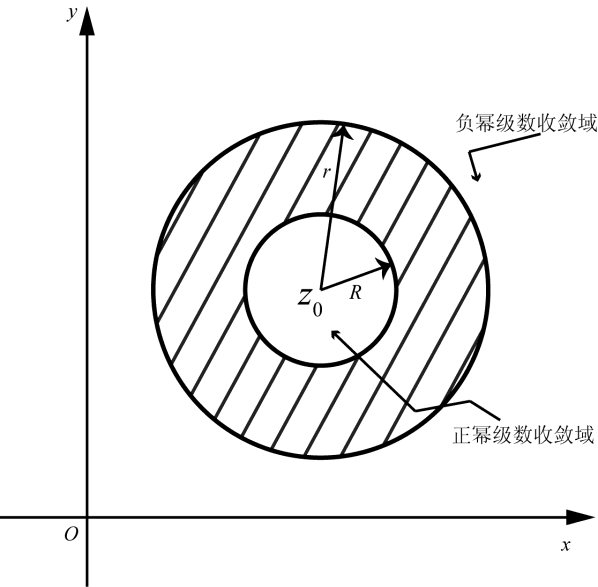
\includegraphics[keepaspectratio,alt={图4.3 洛朗级数：r\textgreater R 时正、负幂级数无公共收敛域}]{figures/04-解析函数的级数表示法/fig-p35-7df0dd55.png}}
\caption{图4.3 洛朗级数：\(r>R\) 时正、负幂级数无公共收敛域}
\end{figure}

\begin{figure}
\centering
\pandocbounded{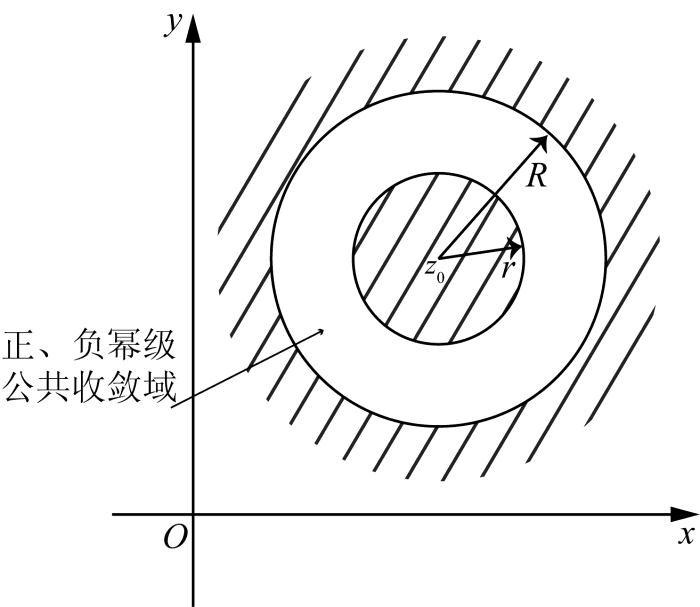
\includegraphics[keepaspectratio,alt={图4.4 洛朗级数：r\textless R 时收敛圆环}]{figures/04-解析函数的级数表示法/fig-p35-e4a70a30.png}}
\caption{图4.4 洛朗级数：\(r<R\) 时收敛圆环}
\end{figure}

\textbf{定理 4.11} 级数
\(\displaystyle\sum_{n=-\infty}^{\infty}a_n(z-z_0)^n\)
在其收敛圆环内的和函数是解析的，而且可以逐项积分和逐项求导数。

\textbf{例 4.6} 讨论级数

\[
\sum_{n=1}^{\infty}\frac{a^n}{z^n}+\sum_{n=0}^{\infty}\frac{z^n}{b^n}
\]

的收敛集，并求和函数，其中 \(a\) 与 \(b\) 为复常数。

\textbf{解} 分别讨论负幂级数和正幂级数。

\textbf{负幂级数}
\(\displaystyle\sum_{n=1}^{\infty}\left(\frac{a}{z}\right)^n\)：当
\(\left|\dfrac{a}{z}\right|<1\)，即 \(|z|>|a|\) 时收敛，且和函数为

\[
\frac{a}{z-a}.
\]

\textbf{正幂级数}
\(\displaystyle\sum_{n=0}^{\infty}\left(\frac{z}{b}\right)^n\)：当
\(\left|\dfrac{z}{b}\right|<1\)，即 \(|z|<|b|\) 时收敛，且和函数为

\[
\frac{b}{b-z}.
\]

（注：正幂级数收敛条件是 \(|z|<|b|\)，这样才能与负幂级数合成圆环
\(|a|<|z|<|b|\)。）

\begin{itemize}
\tightlist
\item
  当 \(|a|<|b|\) 时，原级数收敛且收敛圆环为 \(|a|<|z|<|b|\)，和函数为
\end{itemize}

\[
\frac{a}{z-a}+\frac{b}{b-z}=\frac{(a-b)z}{(a-z)(b-z)} .
\]

\begin{itemize}
\tightlist
\item
  当 \(|a|>|b|\)
  时，负幂级数和正幂级数的收敛域没有公共点，故原级数发散。
\end{itemize}

在圆环 \(|a|<|z|<|b|\) 内解析的函数 \(\dfrac{(a-b)z}{(a-z)(b-z)}\)
可以展开为级数：

\[
\frac{(a-b)z}{(a-z)(b-z)}=\sum_{n=1}^{\infty}\frac{a^n}{z^n}+\sum_{n=0}^{\infty}\frac{z^n}{b^n}.
\]

\subsection{4.4.3 洛朗定理}\label{ux6d1bux6717ux5b9aux7406}

\textbf{定理 4.12} 设 \(f(z)\) 在圆环 \(r<|z-z_0|<R\) 内解析，那么

\[
f(z)=\sum_{n=-\infty}^{\infty}a_n(z-z_0)^n,\qquad r<|z-z_0|<R,
\]

其中

\[
a_n=\frac{1}{2\pi\mathrm{i}}\oint_C\frac{f(\zeta)}{(\zeta-z_0)^{n+1}}\,\mathrm{d}\zeta,\qquad n=0,\pm1,\pm2,\cdots,
\]

这里 \(C\) 为圆环 \(r<|z-z_0|<R\) 内任何一条绕 \(z_0\)
的正向简单闭曲线，且 \(f(z)\) 的表达式是唯一的。

\(f(z)=\displaystyle\sum_{n=-\infty}^{\infty}a_n(z-z_0)^n\ (r<|z-z_0|<R)\)
称为函数 \(f(z)\) 在以 \(z_0\) 为中心的圆环 \(r<|z-z_0|<R\)
内的\textbf{洛朗（Laurent）展开式}。它的右端称为在此圆环内的洛朗级数。

\begin{figure}
\centering
\pandocbounded{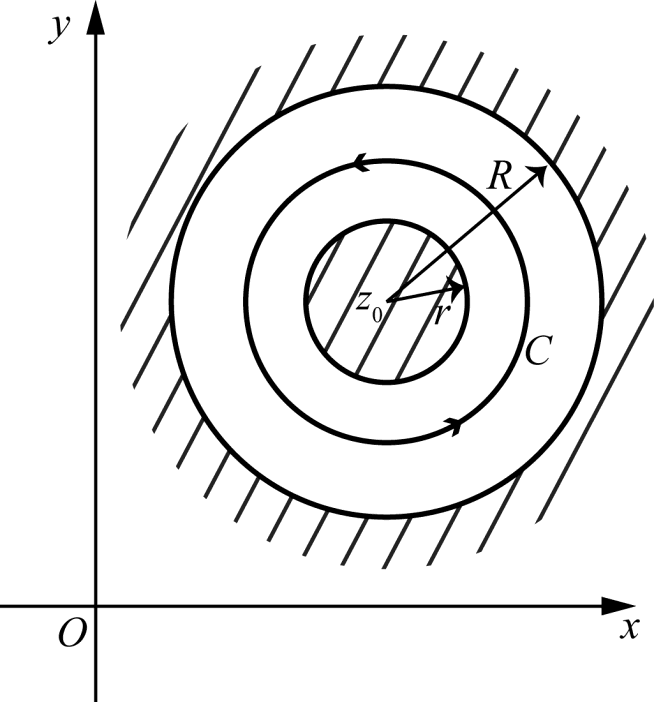
\includegraphics[keepaspectratio,alt={图4.5 洛朗展开的圆环与积分曲线 C}]{figures/04-解析函数的级数表示法/fig-p38-74ee3c5a.png}}
\caption{图4.5 洛朗展开的圆环与积分曲线 \(C\)}
\end{figure}

\textbf{洛朗展开式的唯一性}
所谓洛朗展开式的唯一性，是指函数在某一个给定的圆环的洛朗展开式是唯一的。

\subsection{4.4.4
求洛朗展开的例题}\label{ux6c42ux6d1bux6717ux5c55ux5f00ux7684ux4f8bux9898}

\textbf{例 4.7} 求函数 \(\displaystyle f(z)=\frac{1}{(z-1)(z-2)}\)
在下列圆环内的洛朗级数。

\[
(1)\ 0<|z|<1;\qquad
(2)\ 1<|z|<2;\qquad
(3)\ 2<|z|<+\infty;
\]

\[
(4)\ 0<|z-1|<1;\qquad
(5)\ 1<|z-1|<+\infty .
\]

\textbf{解} 将函数表示成部分分式，有

\[
f(z)=\frac{1}{1-z}-\frac{1}{2-z}.
\]

\textbf{(1)} 在 \(0<|z|<1\) 内，由于 \(|z|<1\)，因此
\(\left|\dfrac{z}{2}\right|<1\)，故

\[
\frac{1}{1-z}=1+z+z^2+\cdots+z^n+\cdots,
\]

\[
\frac{1}{2-z}=\frac{1}{2}\cdot\frac{1}{1-z/2}=\frac{1}{2}\left(1+\frac{z}{2}+\frac{z^2}{4}+\cdots+\frac{z^n}{2^n}+\cdots\right).
\]

于是

\[
f(z)=\left(1+z+z^2+\cdots\right)-\frac{1}{2}\left(1+\frac{z}{2}+\frac{z^2}{4}+\cdots\right)=\sum_{n=0}^{\infty}\left(1-\frac{1}{2^{n+1}}\right)z^n
=\frac{1}{2}+\frac{3}{4}z+\frac{7}{8}z^2+\cdots .
\]

\textbf{(2)} 在 \(1<|z|<2\)
内，\(\left|\dfrac{1}{z}\right|<1\)、\(\left|\dfrac{z}{2}\right|<1\)，故

\[
f(z)=\frac{1}{1-z}-\frac{1}{2-z}=-\frac{1}{z}\cdot\frac{1}{1-1/z}-\frac{1}{2}\cdot\frac{1}{1-z/2}
\]

\[
=-\frac{1}{z}\left(1+\frac{1}{z}+\frac{1}{z^2}+\cdots\right)-\frac{1}{2}\left(1+\frac{z}{2}+\frac{z^2}{4}+\cdots\right)
=-\sum_{n=1}^{\infty}\frac{1}{z^n}-\sum_{n=0}^{\infty}\frac{z^n}{2^{n+1}} .
\]

\textbf{(3)} 在 \(2<|z|<+\infty\)
内，\(\left|\dfrac{1}{z}\right|<1\)、\(\left|\dfrac{2}{z}\right|<1\)，故

\[
f(z)=\frac{1}{1-z}-\frac{1}{2-z}=-\frac{1}{z}\cdot\frac{1}{1-1/z}+\frac{1}{z}\cdot\frac{1}{1-2/z}
\]

\[
=-\frac{1}{z}\left(1+\frac{1}{z}+\frac{1}{z^2}+\cdots\right)+\frac{1}{z}\left(1+\frac{2}{z}+\frac{4}{z^2}+\cdots\right)
=\frac{1}{z^2}+\frac{3}{z^3}+\frac{7}{z^4}+\cdots .
\]

\textbf{(4)} 在 \(0<|z-1|<1\) 内，有

\[
f(z)=\frac{1}{z-2}-\frac{1}{z-1}=-\frac{1}{1-(z-1)}-\frac{1}{z-1}
=-\sum_{n=0}^{\infty}(z-1)^n-\frac{1}{z-1} .
\]

即

\[
f(z)=-\frac{1}{z-1}-1-(z-1)-(z-1)^2-\cdots-(z-1)^n-\cdots .
\]

\textbf{(5)} 在 \(1<|z-1|<+\infty\)
内，\(\left|\dfrac{1}{z-1}\right|<1\)，故

\[
f(z)=\frac{1}{(z-1)-1}-\frac{1}{z-1}=\frac{1}{z-1}\cdot\frac{1}{1-1/(z-1)}-\frac{1}{z-1},
\]

\[
=\frac{1}{z-1}+\frac{1}{(z-1)^2}+\cdots+\frac{1}{(z-1)^n}+\cdots-\frac{1}{z-1}
=\frac{1}{(1-z)^2}+\frac{1}{(z-1)^3}+\cdots+\frac{1}{(z-1)^n}+\cdots .
\]

更简洁地，

\[
f(z)=\sum_{n=2}^{\infty}\frac{1}{(z-1)^n}\qquad(1<|z-1|<\infty).
\]

\subsection{常见错误与注意点}\label{ux5e38ux89c1ux9519ux8befux4e0eux6ce8ux610fux70b9-14}

\begin{itemize}
\tightlist
\item
  洛朗展开的\textbf{收敛域是圆环} \(r<|z-z_0|<R\)，其中 \(r\)
  由负幂级数确定（\(|z-z_0|>r\)），\(R\)
  由正幂级数确定（\(|z-z_0|<R\)）。不要把负幂级数的收敛域也写成圆盘。
\item
  同一个函数在不同的圆环内，洛朗展开式不同；唯一性是指``在给定的某一个圆环内''唯一。
\item
  求洛朗展开一般先做部分分式，再在\textbf{指定的}圆环内选择合适的形式展开：缺项要补
  \(1\)，且必须保证展开所用公比绝对值小于 \(1\)（例 4.7 中分别以
  \(\frac{z}{2}\)、\(\frac{1}{z}\)、\(\frac{2}{z}\)、\(\frac{1}{z-1}\)
  等为公比）。
\item
  例 4.6 中正幂级数 \(\sum(z/b)^n\) 的收敛条件是
  \(|z|<|b|\)（幻灯片上``\(|z|>|b|\)''为笔误），它与负幂级数的
  \(|z|>|a|\) 合成圆环 \(|a|<|z|<|b|\)。
\end{itemize}

\subsection{本节小结}\label{ux672cux8282ux5c0fux7ed3-14}

\begin{itemize}
\tightlist
\item
  洛朗级数是``正幂级数 + 负幂级数''的双向级数，其收敛域一般是圆环
  \(r<|z-z_0|<R\)（还可能是空集、圆盘、圆内去心等退化情形）。
\item
  圆环内解析函数必有洛朗展开，且唯一（定理
  4.12）；系数由围道积分给出，实际求法常用部分分式 + 几何级数。
\item
  圆环内和函数解析，可逐项求导、逐项积分（定理 4.11）。
\item
  洛朗展开是研究孤立奇点分类（§4.5）的直接工具：负幂项的多少决定奇点类型。
\end{itemize}

\section{4.5 孤立奇点}\label{ux5b64ux7acbux5947ux70b9}

\begin{quote}
本节目标：掌握孤立奇点的定义，并能依据洛朗展开式中负幂项的有无与多少，把孤立奇点分成可去奇点、极点、本性奇点三类；掌握极点与零点的关系、本性奇点的刻画（定理
4.14），并会讨论无穷远点的奇点性质。
重点：三类孤立奇点的洛朗级数判别；\(m\) 阶极点与 \(1/f(z)\) 的 \(m\)
阶零点的关系；无穷远点的奇点分类。
难点：负幂项``多少个''与奇点类型的对应；无穷远点作变换 \(z=1/t\)
后的奇点归属；例 4.8 中零极点阶数与可去奇点的判断。
\end{quote}

对应幻灯片：第 43--50 页。

\subsection{4.5.1
孤立奇点的定义与分类}\label{ux5b64ux7acbux5947ux70b9ux7684ux5b9aux4e49ux4e0eux5206ux7c7b}

\textbf{定义 4.4} 若 \(z=z_0\) 为函数 \(f(z)\)
的一个奇点，且存在一个去心邻域 \(0<|z-z_0|<\delta\)，\(f(z)\)
在其中处处解析，则称 \(z_0\) 为 \(f(z)\) 的\textbf{孤立奇点}。

设 \(z_0\) 为 \(f(z)\) 的一个孤立奇点，因为在 \(0<|z-z_0|<\delta\)
中解析，\(f(z)\) 可展开成 \(z-z_0\) 的洛朗级数，即

\[
f(z)=\sum_{n=0}^{\infty}a_n(z-z_0)^n+\sum_{n=1}^{\infty}a_{-n}(z-z_0)^{-n}.
\]

根据洛朗级数中负幂项的情况，把孤立奇点分成三类：

\begin{enumerate}
\def\labelenumi{\arabic{enumi}.}
\tightlist
\item
  级数中不出现负幂项，此时称点 \(z_0\) 为 \(f(z)\) 的\textbf{可去奇点}；
\item
  级数中只含有有限个负幂项，则点 \(z_0\) 称为 \(f(z)\) 的\textbf{极点}；
\item
  级数中含有无穷多个负幂项，点 \(z_0\) 称为 \(f(z)\)
  的\textbf{本性奇点}。
\end{enumerate}

\subsection{4.5.2 可去奇点}\label{ux53efux53bbux5947ux70b9}

\(f(z)\) 在 \(0<|z-z_0|<\delta\) 内的洛朗级数实际为一个幂级数

\[
a_0+a_1(z-z_0)+a_2(z-z_0)^2+\cdots+a_n(z-z_0)^n+\cdots .
\]

这个幂级数在圆盘 \(|z-z_0|<\delta\) 内是收敛的，其和函数为

\[
F(z)=
\begin{cases}
a_0, & z=z_0,\\[4pt]
f(z), & 0<|z-z_0|<\delta .
\end{cases}
\]

\(F(z)\) 在 \(|z-z_0|<\delta\) 内解析。所以不论 \(f(z)\) 原来在 \(z_0\)
是否有定义，我们用 \(F(z)\) 来代替 \(f(z)\)，或令
\(f(z_0)=a_0\)，这样就把奇点除去了。由于这个原因，所以 \(z_0\)
称为可去奇点。

\subsection{4.5.3 极点}\label{ux6781ux70b9}

设 \(z=z_0\) 为函数 \(f(z)\) 的极点。若 \(f(z)\) 在 \(0<|z-z_0|<\delta\)
内洛朗展开式为

\[
f(z)=\frac{a_{-m}}{(z-z_0)^m}+\cdots+\frac{a_{-1}}{z-z_0}+\sum_{n=0}^{\infty}a_n(z-z_0)^n,\qquad(m\ge 1,\ a_{-m}\neq 0),
\]

则称 \(z_0\) 为 \(f(z)\) 的 \(m\) 阶极点。

此时可写成

\[
f(z)=\frac{1}{(z-z_0)^m}\varphi(z),
\]

其中

\[
\varphi(z)=a_{-m}+a_{-m+1}(z-z_0)+a_{-m+2}(z-z_0)^2+\cdots+a_{-1}(z-z_0)^{m-1}+\sum_{n=0}^{\infty}a_n(z-z_0)^{n+m},
\]

\(\varphi(z)\) 在 \(|z-z_0|<\delta\) 内解析且
\(\varphi(z_0)=a_{-m}\neq 0\)。反之，若有在 \(|z-z_0|<\delta\)
内解析且在 \(z_0\) 处函数值不为零的函数
\(\varphi\)，使得上面这种洛朗展开式成立，则容易看出 \(z_0\) 为 \(f(z)\)
的 \(m\) 阶极点。

\textbf{定理 4.13} 如果 \(z_0\) 是 \(f(z)\) 的 \(m\) 阶极点，那么
\(z_0\) 就是 \(\dfrac{1}{f(z)}\) 的 \(m\) 阶零点。反过来也成立。

\subsection{4.5.4 本性奇点}\label{ux672cux6027ux5947ux70b9}

\textbf{定理 4.14（Weierstrass 定理）} 如果 \(z_0\) 为 \(f(z)\)
的本性奇点，那么对于任意给定的复数 \(A\)，总可以找到一个趋于 \(z_0\)
的数列 \(\{z_n\}\)，使得

\[
\lim_{n\to\infty}f(z_n)=A .
\]

\(f(z)\) 的孤立奇点 \(z_0\) 的邻域中，按可去奇点、极点、本性奇点的顺次有

\[
(1)\ \lim_{z\to z_0}f(z)=\text{有限数};
\]

\[
(2)\ \lim_{z\to z_0}f(z)=\infty;
\]

\[
(3)\ \lim_{z\to z_0}f(z)\ \text{不存在}.
\]

\subsection{4.5.5
函数在无穷远点的性质}\label{ux51fdux6570ux5728ux65e0ux7a77ux8fdcux70b9ux7684ux6027ux8d28}

如果函数 \(f(z)\) 是在无穷远点 \(z=\infty\) 的去心邻域 \(R<|z|<\infty\)
内解析，那么称点 \(\infty\) 为 \(f(z)\) 的孤立奇点。

作变换 \(\displaystyle z=\frac{1}{t}\)，记
\(\displaystyle g(t)=f\left(\frac{1}{t}\right)\)，则 \(g(t)\) 在
\(0<|t|<\frac{1}{R}\) 中解析，即 \(t=0\) 是 \(g(t)\) 的孤立奇点。

如果 \(t=0\) 是 \(g(t)\) 的可去奇点、\(m\)
阶极点或是本性奇点，那么就称点 \(z=\infty\) 是 \(f(z)\)
的可去奇点、\(m\) 阶极点或本性奇点。

因为 \(g(t)\) 在原点的邻域内有洛朗展式：

\[
g(t)=\sum_{n=-\infty}^{\infty}a_n t^n,\qquad 0<|t|<\frac{1}{R},
\]

所以 \(f(z)\) 在 \(R<|z|<\infty\) 中有下面的洛朗展式

\[
f(z)=\sum_{n=-\infty}^{\infty}b_n z^n,\qquad R<|z|<\infty,
\]

其中

\[
b_n=a_{-n}\ (n=0,\pm1,\pm2,\cdots),\qquad
b_n=\frac{1}{2\pi\mathrm{i}}\oint_C\frac{f(\zeta)}{\zeta^{n+1}}\,\mathrm{d}\zeta,\qquad n=0,\pm1,\pm2,\cdots,
\]

其中 \(C\) 为圆环域 \(R<|z|<\infty\) 内绕原点的任何一条正向简单闭曲线。

在级数
\(f(z)=\displaystyle\sum_{n=-\infty}^{\infty}b_n z^n\ (R<|z|<\infty)\)
中：

\begin{enumerate}
\def\labelenumi{\arabic{enumi}.}
\tightlist
\item
  不含正幂项 \(\iff\) \(\infty\) 为可去奇点 \(\iff\)
  \(\lim_{z\to\infty}f(z)\) 存在；
\item
  含有有限多个正幂项，且 \(z^m\) 为最高正幂 \(\iff\) \(\infty\) 为 \(m\)
  阶极点 \(\iff\) \(\lim_{z\to\infty}f(z)=\infty\)；
\item
  含有无穷多正幂项 \(\iff\) \(\infty\) 为本性奇点 \(\iff\)
  \(\lim_{z\to\infty}f(z)\) 不存在。
\end{enumerate}

\subsection{4.5.6 例题}\label{ux4f8bux9898-3}

\textbf{例 4.8} 函数
\(\displaystyle f(z)=\frac{(\mathrm{e}^z-1)(z-2)^4}{(\sin\pi z)^4}\)
在扩充的复平面上有无奇点？是什么类型？若是极点，求出其阶。

\textbf{解} 函数有奇点 \(0,\pm1,\pm2,\cdots\) 和
\(\infty\)。这是因为函数在这些点无定义，所以是奇点。

\textbf{(1)} \(z=0\) 是 \(\sin\pi z\) 的一阶零点，从而是
\((\sin\pi z)^4\) 的四阶零点；但它又是分子 \(\mathrm{e}^z-1\)
的一阶零点（因为 \(\mathrm{e}^z-1\) 在 \(z=0\) 处为零且导数
\(\mathrm{e}^0=1\neq 0\)），故 \(z=0\) 是函数的三阶极点（\(4-1=3\)）。

\textbf{(2)} 同 (1)，\(\pm1,-2,\pm3,\pm4,\cdots\) 是函数的四阶极点（对
\(k\neq 0,2\)，分子 \((\mathrm{e}^k-1)(k-2)^4\neq 0\)，而
\((\sin\pi k)^4\) 为四阶零点）。

\textbf{(3)} \(z=2\) 是可去奇点。

\[
\lim_{z\to2}f(z)=\lim_{z\to2}(\mathrm{e}^z-1)\cdot\lim_{z\to2}\left(\frac{z-2}{\sin\pi z}\right)^4
=(\mathrm{e}^2-1)\cdot\frac{1}{\pi^4}.
\]

因为
\(\lim_{z\to2}\dfrac{z-2}{\sin\pi z}=\dfrac{1}{\pi\cos 2\pi}=\dfrac{1}{\pi}\)，所以极限为有限数，故
\(z=2\) 为可去奇点。

\textbf{(4)} 考察 \(\infty\)：令 \(z=1/t\)，则

\[
f\left(\frac{1}{t}\right)=\frac{(\mathrm{e}^{1/t}-1)(1-2t)^4}{t^4\left(\sin\dfrac{\pi}{t}\right)^4}.
\]

所以 \(t=0\) 及 \(t_n=\dfrac{1}{n}\ (n=1,2,\cdots)\) 均为上式的奇点。当
\(n\to\infty\) 时，\(t_n\to0\)，所以 \(t=0\) 不是 \(f(1/t)\)
的孤立奇点，也就是说 \(z=\infty\) 不是 \(f(z)\) 的孤立奇点。

\subsection{常见错误与注意点}\label{ux5e38ux89c1ux9519ux8befux4e0eux6ce8ux610fux70b9-15}

\begin{itemize}
\tightlist
\item
  判断奇点类型必须\textbf{先看洛朗展开式中负幂项}：无负幂项（可去）、有限个负幂项（极点）、无穷多个负幂项（本性奇点）。
\item
  ``\(m\) 阶零点''与``\(m\) 阶极点''互为倒数的关系（定理
  4.13）非常常用：分子零点阶数与分母零点阶数相减即得极点阶数（例 4.8）。
\item
  若分子、分母在同一零点处都有零点，要相抵（如 \(z=2\)：分子 \((z-2)^4\)
  四阶零点与分母 \((\sin\pi z)^4\) 四阶零点抵消，成为可去奇点）。
\item
  无穷远点必须先作变换 \(z=1/t\) 化为原点 \(t=0\) 研究；并根据 \(g(t)\)
  的洛朗级数（即 \(f(z)\) 的级数中\textbf{正幂项}）来判别。
\item
  记法：对无穷远点，正幂项（\(z^n,\ n>0\)）的多少对应 \(\infty\)
  的奇点类型，与有限孤立奇点看负幂项正好对偶。
\end{itemize}

\subsection{本节小结}\label{ux672cux8282ux5c0fux7ed3-15}

\begin{itemize}
\tightlist
\item
  孤立奇点由去心邻域内解析定义（定义 4.4），其洛朗级数负幂项决定类型。
\item
  可去奇点：无负幂项，可通过补充定义值 \(f(z_0)=a_0\) 使函数解析。
\item
  \(m\) 阶极点：负幂项最高为 \((z-z_0)^{-m}\)，等价于
  \(f(z)=\dfrac{\varphi(z)}{(z-z_0)^m}\)，\(\varphi(z_0)\neq 0\)；且
  \(z_0\) 是 \(1/f(z)\) 的 \(m\) 阶零点（定理 4.13）。
\item
  本性奇点：无穷多个负幂项；由定理 4.14，其极限不存在（且值在 \(z_0\)
  附近任意接近任何复数 \(A\)）。
\item
  无穷远点的奇点性质通过 \(z=1/t\) 转化为原点奇点研究；正幂项决定
  \(\infty\) 的类型（§4.5.5）。
\end{itemize}

\newpage
